\documentclass[a4paper, 12pt, british]{article} % aritcle

% make the page text 17cm wide, 24cm high
\usepackage[a4paper, total={17cm, 24cm}]{geometry}

\usepackage{amsmath}    % need for subequations
\usepackage{amssymb}    % this has \therefore
\usepackage{graphicx}   % need for figures
\usepackage{verbatim}   % useful for program listings
\usepackage{color}      % use if color is used in text
\usepackage{caption}
\usepackage{subcaption}
%\usepackage{subfigure}  % use for side-by-side figures
\usepackage{hyperref}   % use for hypertext links, including those to external documents and URLs
\usepackage{tabularx}
\usepackage{float}
\usepackage{enumitem}
\usepackage[useregional]{datetime2}

% must use lualatex to use these two
%\usepackage{fontspec}
%\setmainfont{Times}

\usepackage{fancyhdr}
\pagestyle{fancy} 
\lhead[\fancyplain{}{\bfseries\thepage}]{\fancyplain{}
	{\let\uppercase\relax\rightmark}}
\rhead[\fancyplain{}{\let\uppercase\relax\leftmark}]{\fancyplain{}
	{\bfseries\thepage}}
\cfoot[\fancyplain{}{}]{\fancyplain{}{}}


\usepackage{tocstyle}
\usetocstyle{classic}
\setcounter{secnumdepth}{3}
\setcounter{tocdepth}{2}

\numberwithin{equation}{section}
\numberwithin{figure}{section}
\numberwithin{table}{section}

% paragraph indent
\setlength{\parindent}{2em}
\setlength{\parindent}{0pt}
% paragraph spacing
\setlength{\parskip}{0.5em}

\title{CIVE2470: Water Engineering and geotechnics\\ \quad \\An Introduction to Open Channel Hydraulics}
\author{Dr Andrew Sleigh\\School of Civil Engineering\\University of Leeds}
\date{February 2020 \\ \quad \\{\scriptsize This version was created on:\\ \DTMnow}}


\begin{document}

\maketitle

\tableofcontents


\newpage 
\section{Basic Equations of Open Channel Hydraulics}
\subsection{Definition and differences between pipe flow and open channel flow}
Open-channel hydraulics, or Open Channel Flow, is an important area of fluid mechanics for civil engineers. It describes the flow in rivers, man-made channels and partially-full pipes, as well as the behaviour of hydraulic structures such as weirs, spillways and sluices. 

The common feature of all open-channel flows is the free surface, subject to atmospheric pressure, in other words with a gauge pressure $p = 0$. All such flows are \textit{gravity-driven}, with the discharge and flow depth $y$ dependent on the balance between the downslope component of gravity and bed friction.

Pressurised Pipe flow and Open Channel flow are similar in many ways but differ in one important respect. 
\begin{figure}[H]
	\centering
	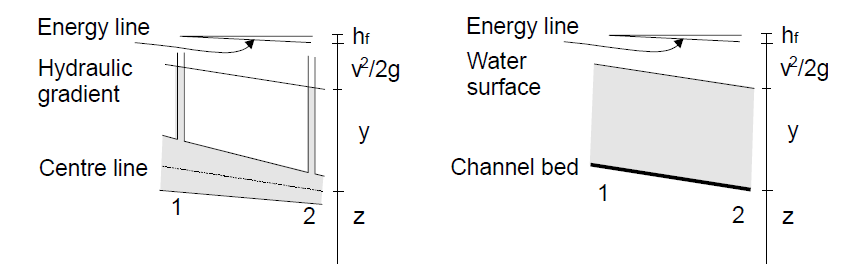
\includegraphics[scale=0.6]{./images/fig_11.png}
	\caption{Figure of pipe and open channel flow}
	\label{fig:111}
\end{figure}


The two kind of flow are compared in figure \ref{fig:111} above. On the left is pipe flow. Two piezometers are placed in the pipe at sections 1 and 2. The water levels in the pipes are maintained by the pressure in the pipe at elevations represented by the hydraulics grade line or hydraulic gradient. The pressure exerted by the water in each section of the pipe is shown in the tube by the height y of a column of water above the centre line of the pipe.

The total energy of the flow of the section (with reference to a datum) is the sum of the elevation $z$ of the pipe centre line, the piezometric head $y$ and the velocity head $V^2/2g$ , where $V$ is the mean velocity. The energy is represented in the figure by what is known as the \textit{energy grade line} (sometimes reffered to as the \textit{energy gradient}).

The loss of energy that results when water flows from section 1 to section 2 is represented by $h_f$.

A similar diagram for open channel flow is shown to the right. This is simplified by assuming parallel flow with a uniform velocity distribution and that the slope of the channel is small. In this case the hydraulic gradient is the water surface as the depth of water corresponds to the piezometric height.

Despite the similarity between the two kinds of flow, it is much more difficult to solve problems of flow in open channels than in pipes. Flow condition in open channel are complicated by the position of the free surface which is likely to change with time and space. And also by the fact that depth of flow, the discharge, and the slopes of the channel bottom and of the free surface are all inter dependent.

Physical conditions in open-channels vary much more than in pipes - the cross-section of pipes is usually round - but for open channel it can be any shape.

Treatment of roughness also poses a greater problem in open channels than in pipes. Although there may be a great range of roughness in a pipe from polished metal to highly corroded iron, open channels may be of polished metal to natural channels with long grass and roughness that may also depend on depth of flow.

Open channel flows are found in large and small scale. For example the flow depth can be between a few cm in water treatment plants and over $10m$ in large rivers. The mean velocity of flow may range from less than $0.01 m/s$ in tranquil waters to above $50 m/s$ in high-head spillways. The range of total discharges may extend from $0.001 l/s$ in chemical plants to greater than $10000 m^3/s$ in large rivers or spillways. 

In each case the flow situation is characterised by the fact that there is a \textbf{free surface} whose position is \textbf{NOT known beforehand} - it is determined by applying momentum and continuity principles.

In general the treatment of open-channel flow is more empirical than pipe flow - but can still produce useful results.

Table \ref{tab:11} summarises the similatities and differences between Pipe flow and Open Channel flow.

\begin{table}[H]
	\centering
	\begin{tabularx}{\textwidth}{lXX}
		\hline
		\noalign{\vskip 2mm} 
		   & \textbf{Pipe Flow} & \textbf{Open Channel Flow}  \\ 
		\hline
		\noalign{\vskip 2mm} 
Flow driven by&	Pressure work&	Gravity (potential energy)\\
		\hline
Flow cross section &	Known, fixed&	Unknown in advance because the flow depth is unknown\\
		\hline
Characteristic flow parameters&	velocity deduced from continuity&	Flow depth deduced simultaneously from solving both continuity and momentum equations\\
		\hline
Specific boundary conditions& &		Atmospheric pressure at the free surface\\
		\hline
	\end{tabularx}
	\caption{Differences Between Pipe Flow and Open Channel FLow}
	\label{tab:11}
\end{table}


\newpage
\subsection{Types of flow / Classification of flow}

Open-channel flow is steady if all flow properties are independent of time. The most important examples of unsteady flow are waves, surges and tidal flows. In this part of the course we consider only \textbf{steady flow}. 

Within the category of steady flow there are several classifications that are useful for identifiing situations where dirreerent analysis must be applied. 

The figure and text below discusses these classifications.

\begin{figure}[H]
	\centering
	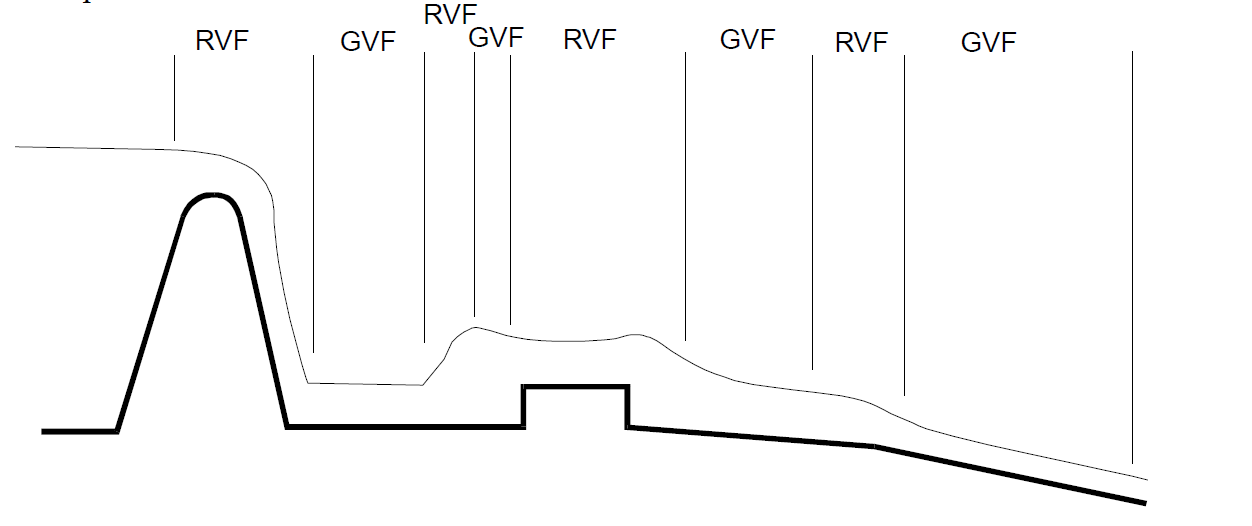
\includegraphics[scale=0.5]{./images/fig_12.png}
	\caption{Types of flow that may occur in open channels}
	\label{fig:121}
\end{figure}


\begin{itemize}


\item\textbf{Uniform flow: UF}\\
In uniform flow the depth and cross-stream velocity profile do not vary in the direction of flow. This can only occur in a long straight channel of uniform cross section, constant slope and no side streams. (These are called \textit{prismatic channels}; they are always an approximation for natural water courses like rivers). In uniform flow the downslope component of weight exactly balances bed friction. Steady uniform flow is also called \textbf{\textit{normal flow}}. All steady downslope flows in uniform channels tend to normal flow if there is sufficient distance. 

\item \textbf{Gradually Varied Flow: GVF}\\
In gradually-varied flow the water depth changes slowly with streamwise distance (typically over distances of hundreds or thousands of times the flow depth) because of an imbalance between gravitational and friction forces. This may occur as the result of a change in channel conditions (slope, cross-section or roughness) or as an adjustment brought about by upstream or downstream disturbances such as weirs and sluices. Because the variation is gradual the flow can still be treated as \textit{one-dimensional} (varying only with $x$) and the pressure as \textit{hydrostatic}.  

\item \textbf{Rapidly Varied Flow: RVF}\\
Rapidly-varied flow occurs when the flow adjusts over relatively short distances (a few times the flow depth). Examples are hydraulic jumps, as well as flow past hydraulic structures such as weirs, venturis (local narrowing) and sluices. As the streamwise distance is relatively short, the rapid changes to flow properties can often by obtained by neglecting bed friction.
\end{itemize}

\subsection{Properties  of open channels }

\textbf{Artificial channels}\\
These are channels that have been constructed. They include irrigation canals, navigation canals, spillways, sewers, culverts and drainage ditches. They are usually constructed in a regular cross-section shape throughout - and are thus prismatic channel (they don't widen or get narrower along the channel). In the field they are commonly constructed of concrete, steel or earth and have the surface roughness- reasonably well defined (although this may change with age - particularly grass lined channels.) Analysis of flow in such well-defined channels will give reasonably accurate results.

\textbf{Natural channels}\\
Natural channels can be very different fro each other. They are not regular nor prismatic and their materials of construction can vary widely (although they are mainly of earth this can possess many different properties.) The surface roughness will often change with time distance and even elevation. Consequently it becomes more difficult to accurately analyse and obtain satisfactory results for natural channels than is does for artificial ones. 

\subsubsection{Geometric properties necessary for analysis}
For analysis various geometric properties of the channel cross-sections are required. For artificial channels these can usually be defined using simple algebraic equations that are functions of$y$, the depth of flow. 

Consider the general section and notation shown in figure \ref{fig:section_general_0}
\begin{figure}[H]
	\centering
	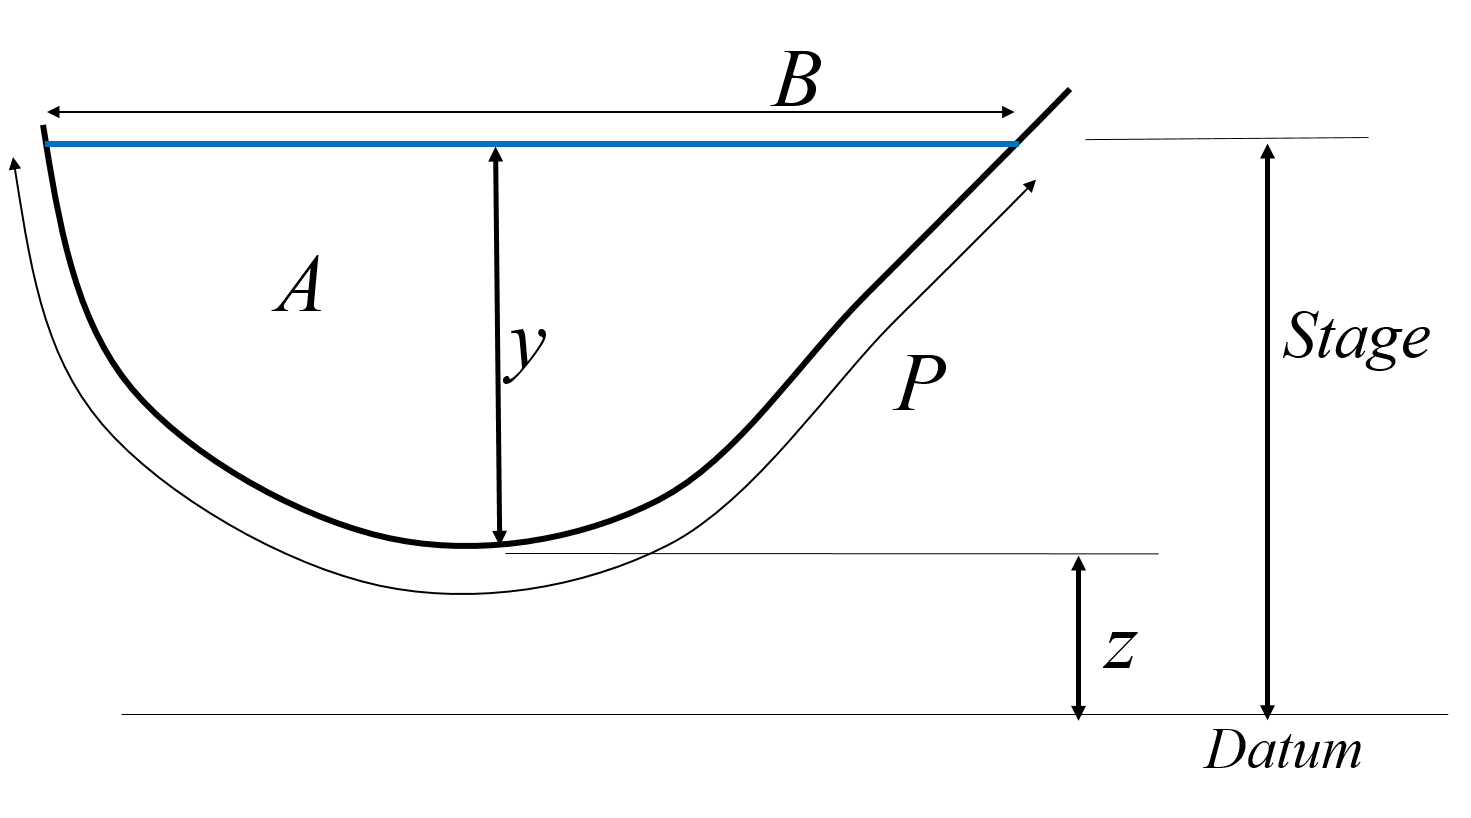
\includegraphics[width=10cm]{./images/section_general.png}
	\caption{A general section of a channel with notation}
	\label{fig:section_general_0}
\end{figure}

The commonly needed geometric properties are defined as:
\begin{itemize}
	\item Depth ($y$) - the vertical distance from the lowest point of the channel section to the free surface.
\item Stage ($z$) - the vertical distance from the free surface to an arbitrary datum
\item Area ($A$) - the cross-sectional area of flow, normal to the direction of flow
\item Wetted perimeter ($P$) - the length of the wetted surface measured normal to the direction of flow.
\item Surface width ($B$) - width of the channel section at the free surface
\item Hydraulic radius ($R$) - the ratio of area to wetted perimeter (A/P)
\item Hydraulic mean depth ($D_m$) (or sometimes $\delta$) - the ratio of cross-sectional area to surface width $(A/B)$
\end{itemize}

For common channel shapes it is possible to derive formulae that enable these to be calculated as function of the depth and other geometric measures. These formulae are straight-forward to derive, but is is usefuul to have them handy for reference, as in table \ref{tab:131}.
\begin{table}[H]
	\centering
	\begin{tabularx}{\textwidth}{lccc}
		\hline
		\noalign{\vskip 2mm} 
		 & Rectangle & Trapezoid & Circle \\
		 \hline
		 \noalign{\vskip 2mm} 
		& 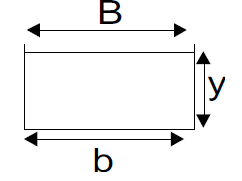
\includegraphics[scale=0.5]{./images/fig_131a.png}&  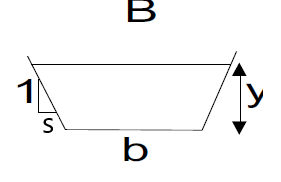
\includegraphics[scale=0.5]{./images/fig_131b.png}& 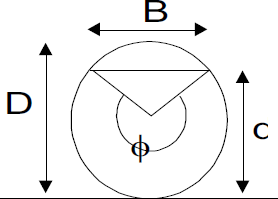
\includegraphics[scale=0.5]{./images/fig_131c.png} \\ 
						& &  & ($\phi$ in \textit{radians}) \\ 
		\hline
		\noalign{\vskip 2mm} 
		 Area, $A$ & $by$ &$(b+sy)y$ & $\frac{1}{8}(\phi - \sin \phi)D^2$ \\
		 		\hline
		 \noalign{\vskip 2mm} 
		 Wetted perimeter, $P$ &$b+2y$& $b+2y\sqrt{1+s^2}$& $\frac{1}{2}\phi D$\\
		 		\hline
		 \noalign{\vskip 2mm} 
		 Top width, $B$ &$b$ & $b+2sy$ & $(\sin(\phi/2))D$ \\
		 		\hline
		 \noalign{\vskip 2mm} 
		 Hydraulic Radius, $R = \frac{A}{P}$ & $\frac{by}{b+2y}$&$ \frac{(b+sy)y}{b+2y\sqrt{1+x^2}}$ & $\frac{1}{4}\left(1-\frac{\sin \phi}{\phi}\right)D$ \\
		 		\hline
		 \noalign{\vskip 2mm} 
		 Hydraulic mean depth, $D_m = \frac{A}{B}$ & $y$&$\frac{(b+sy)y}{b+2sy}$ & $\frac{1}{8}\left(\frac{\phi - \sin \phi}{\sin (\phi/2)}\right)D$\\
\hline
	\end{tabularx}
	\caption{Equations of Section Properties for Rectangular, Trapezoidal and Circular sections}
	\label{tab:131}
\end{table}


\subsection{Fundamental equations}

The equations which describe the flow of fluid are derived from three fundamental laws of physics:

\begin{enumerate}
	\item Conservation of matter (or mass)
\item Conservation of energy 
\item Conservation of momentum
\end{enumerate}

In solid mechanics these laws may be applied to an object which is has a fixed shape and is clearly defined. In fluid mechanics the object is not clearly defined and as it may change shape constantly. To get over this we use the idea of  \textit{control volumes}. These are imaginary volumes of fluid within the body of the fluid. To derive the basic equation the above conservation laws are applied by considering the forces applied to the edges of a control volume within the fluid. Figure \ref{fig:141} shows a short length of channel used as the control voume for open channel flow analysis. 
 
 \begin{figure}[H]
 	\centering
 	%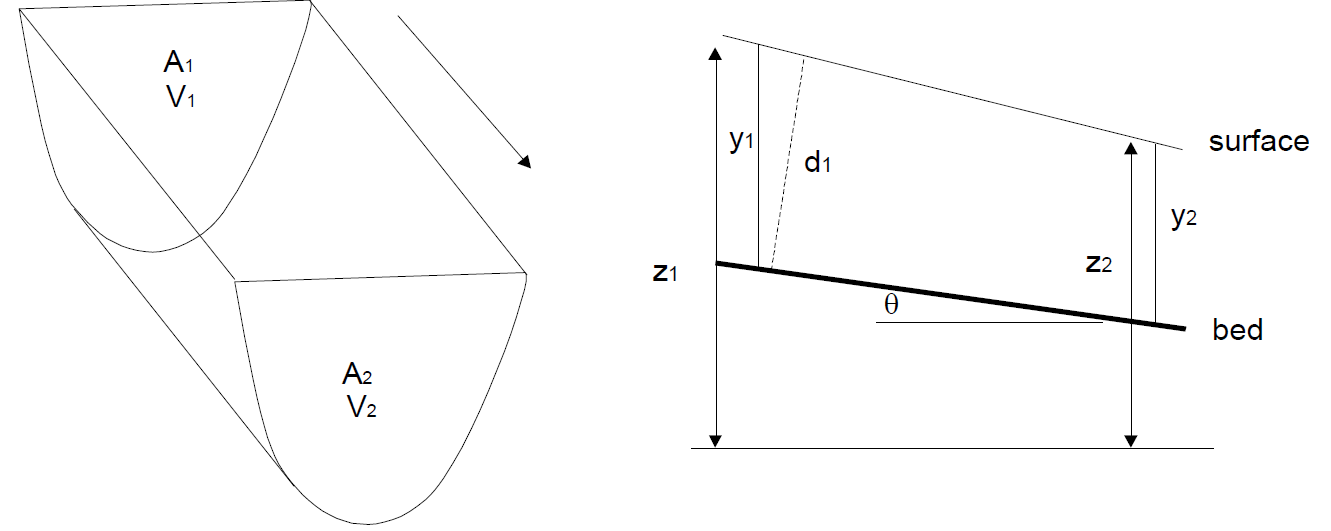
\includegraphics[scale=0.45]{./images/fig_141.png}
 	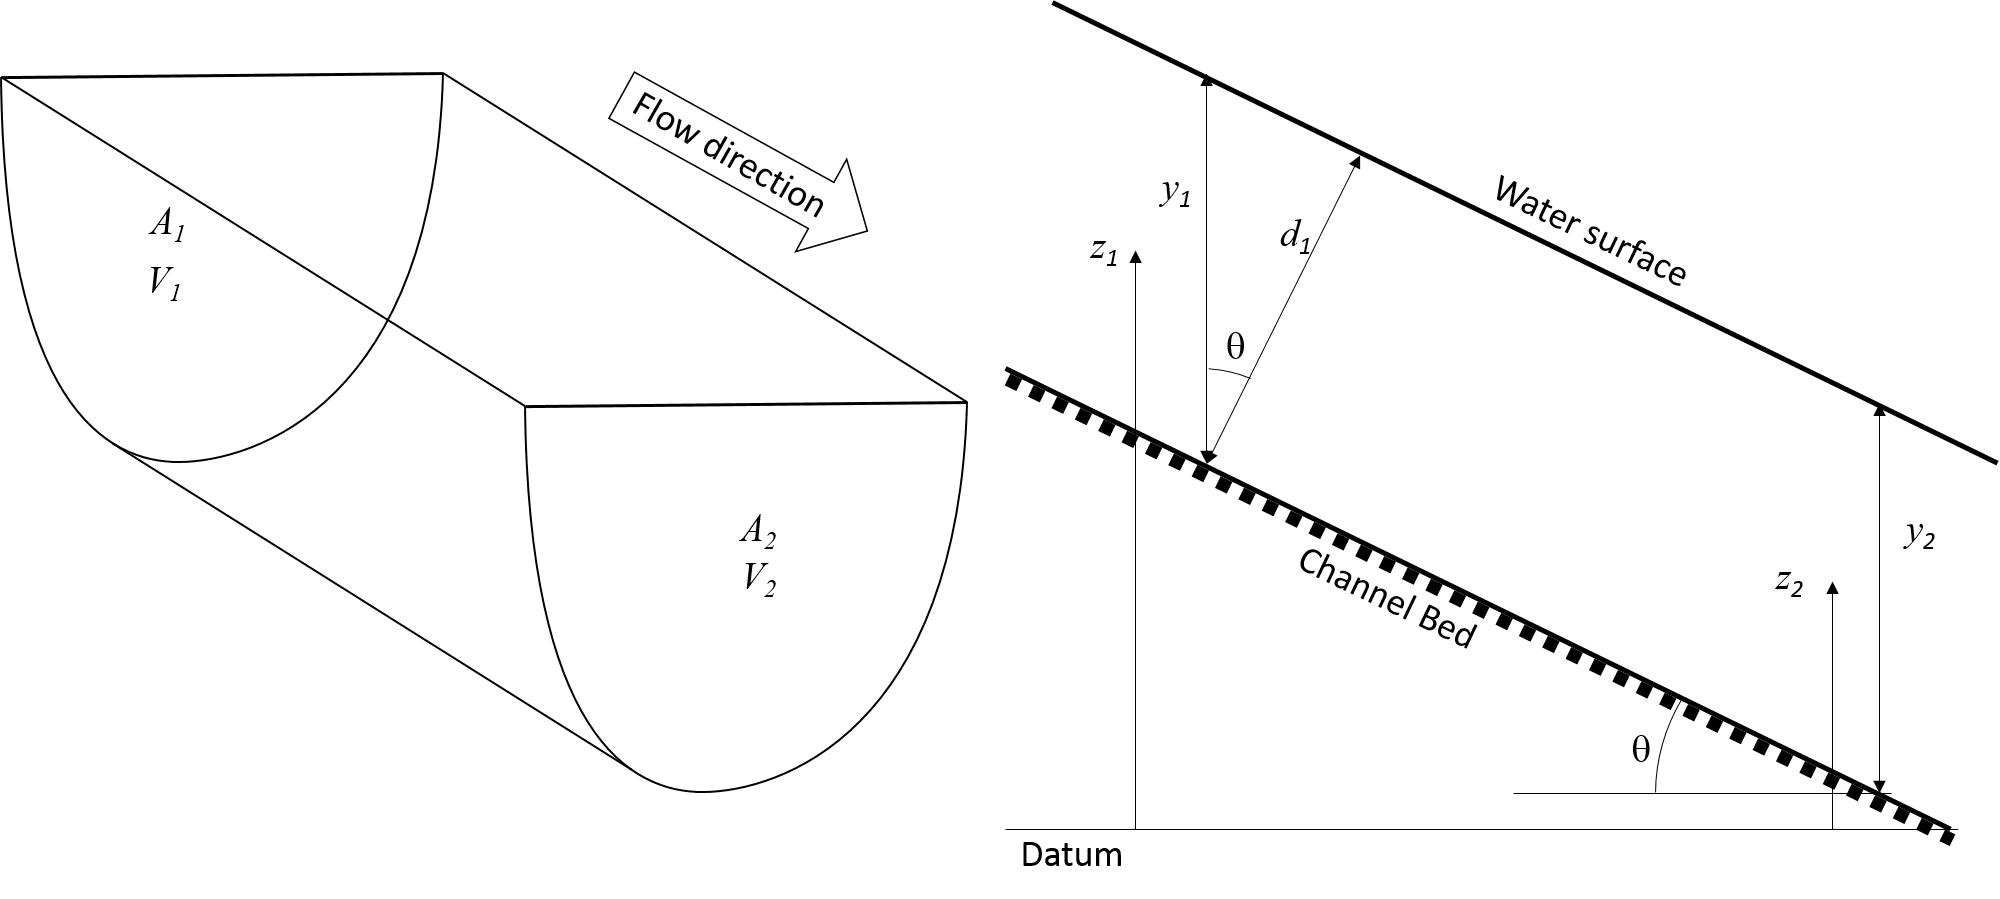
\includegraphics[scale=0.45]{./images/channel_cv_2018.png}
 	\caption{A small length of channel as a control volume}
 	\label{fig:141}
 \end{figure}

\subsubsection{The Continuity Equation (conservation of mass) for Open Channel Flow}
For any control volume during the small time interval $\delta t$ the principle of conservation of mass implies that the mass of flow entering the control volume minus the mass of flow leaving the control volume equals the change of mass within.

If the flow is steady and the fluid incompressible the mass entering is equal to the mass leaving, so there is no change of mass within the control volume.  So for the time interval $\delta t$:
\begin{equation*}
\text{Mass flow entering} = \text{mass flow leaving}
\end{equation*}

Considering the control volume above which is a short length of open channel of arbitrary cross-section then, if $\rho$ is the fluid density and $Q$ is the volume flow rate then
mass flow rate is $\rho Q$ and the continuity equation for steady incompressible flow can be written

 \begin{equation*}
\rho Q_\text{entering} = \rho Q_\text{leaving}
\end{equation*} 

As, $Q$, the volume flow rate is the product of the area and the mean velocity ($Q=VA$) then (cancelling the $\rho$), the continuity equation can be written as

\begin{equation}
V_1 A_1 = V_2 A_2
 \end{equation}


\subsubsection{The Energy equation (conservation of energy) for Open Channel Flow}

We have seen the Energy Euation several time before it is the familiar \textbf{}Bernoulli equation as - the statement of conservation of energy. Applying this between the two cross-sections of the control volumne
would give:
 \begin{equation}
\frac{p_1}{\rho_1 g}  + \frac{V_1^2}{2g} + z_1  = \frac{p_2}{\rho_2 g}  + \frac{V_2^2}{2g} + z_2 = H = \text{constant}
\label{eq:bernoulli}
 \end{equation}

In this derivation it was assumed that no energy is lost in the control volume - i.e. the fluid is frictionless. To apply to \textit{situation with friction} some energy  loss term must be included

For application to Open Channel flow we can write $p = \rho g y$ so the term 
$\frac{p}{\rho g}=\frac{\rho g y}{\rho g} = y$ which results in the Bernoulli equation being written: 
\begin{equation}
y_1  + \frac{V_1^2}{2g} + z_1  = y_2  + \frac{V_2^2}{2g} + z_2 = H = \text{constant}
\label{eq:bernoulli_y}
\end{equation}
This is the Bernoulli Equation we will use for analysis of Open Channel Flow.

\subsubsection{The momentum equation (momentum principle) for Open Channel Flow}

Again consider the control volume above during the time $\delta t$
 \begin{align*}
\text{momentum entering} &= \rho \delta Q_1 \: \delta t\: V_1 \\
\text{momentum leaving} &= \rho \delta Q_2 \; \delta t\; V_2
\label{eq:momentum_principal}
\end{align*}
 

By the continuity principle : $\delta Q_1 = \delta Q_2 = \delta Q$
And by Newton's second law Force = rate of change of momentum

 \begin{align*}
\delta F &= \frac{\text{momentum leaving - momentum entering}}{\delta t} \nonumber\\ 
 &= \rho \: \delta Q(V_2 - V_1)
\end{align*}
 

\begin{equation}
F = \rho \:  Q(V_{2} - V_{1})
\end{equation}

This is the momentum equation for steady flow for a region of uniform velocity.

\subsubsection{Energy and Momentum coefficients}

In deriving the above momentum and energy (Bernoulli) equations it was noted that the velocity must be constant (equal to $V$) over the whole cross-section or constant along a stream-line. Clearly this will not occur in practice.  Fortunately both these equation may still be used even for situations of quite non-uniform velocity distribution over a section. This is possible by the introduction of coefficients of energy and momentum, $\alpha$ and $\beta$ respectively.

These are defined:

\begin{equation}
\alpha = \frac{\int \rho u^3 \; dA}{\rho V^3 A}
\label{eq:alpha}
\end{equation} 


 \begin{equation}
 \beta = \frac{\int \rho u^2 \; dA}{\rho V^2 A}
 \label{eq:beta}
 \end{equation} 
where $V \; (=Q/A)$ is the mean velocity.

And the Bernoulli equation, Eqn \ref{eq:bernoulli_y}, can be rewritten in terms of this mean velocity:
 \begin{equation}
y  + \frac{ \alpha V^2}{2g} + z  = H = \text{constant}
\label{eq:bernoulli_V}
\end{equation}
 

And the general momentum equation becomes:
 \begin{equation}
 F = \rho \:  Q \; \beta(V_{2} - V_{1})
 \label{eq:momentum_gen}
 \end{equation}


The values of $\alpha$ and $\beta$ must be derived from the velocity distributions across a cross-section. They will always be greater than 1, but only by a small amount consequently they can often be confidently omitted - but not always and their existence should always be remembered. For turbulent flow in regular channel $\alpha$ does not usually go above 1.15 and $\beta$ will normally be below 1.05. 

\subsection{Laminar and Turbulent flow}

As in pipes, and all flow, the flow in an open channel may be either laminar or turbulent. The criterion for determining the type of flow is the Reynolds Number, $R_e$.

For pipe flow (where $D$ is pipe diameter)
\begin{equation}
R_e = \frac{\rho V D}{\mu} = \frac{VD}{\nu}
\label{eq:re}
\end{equation} 
And the limits for reach type of flow are
\begin{align*}
\text{Laminar}&:  R_{e \text{ pipe}} < 2000 \\
\text{Turbulent}&:  R_{e \text{ channel}} > 4000
\end{align*}

If we take the characteristic length as the hydraulic radius $R = A/P$ then for a pipe \underline{flowing full} 
\begin{equation*}
R = \frac{\pi D^2/4}{\pi D}=\frac{D}{4} 
\end{equation*}
and
\begin{equation}
R_e = \frac{\rho V R}{\mu}=\frac{\rho V}{\mu}\frac{D}{4} = \frac{R_{e  \text{ pipe}}}{4} 
\end{equation}


So for an open channel the limits for each type of flow become
\begin{align*}
\text{Laminar}&:  R_{e \text{ channel}} < 500 \\
\text{Turbulent}&:  R_{e \text{ channel}} > 1000
\end{align*}


In practice the limit for turbulent flow is not so well defined in channel as it is in pipes and so 2000 is often taken as the threshold for turbulent flow.

%We can draw further from pipe flow analysis to look at the effect of friction. Taking the Darcy-Wiesbach formula for head loss due to friction in a pipe in turbulent flow 
%
%\begin{equation}
%h_f = \frac{4fLV^2}{2gD}
%\end{equation}
%
%and make the substitution for hydraulic radius $R = D/4 $,
%and if we put the bed slope $S_o = L/h_f$ then
%
%\begin{align}
% S_o = \frac{L}{h_f} \nonumber \\
% S_o = \frac{4fV^2}{2g \; 4R}
%\end{align}
% 
%and
%\begin{equation}
%\lambda = \frac{8gRS_o}{V^2} \qquad \qquad f = \frac{2gRS_o}{V^2}
%\end{equation}
%
%  
%
%The \textit{Colebrook-White}  equation gives the $f - R_e$ relationship for pipes, putting in $R=D/4$ the equivalent equation for open channel is
%
% \begin{equation}
%\frac{1}{\sqrt{f}} = -4 \log_{10} \left(\frac{k_s}{14.8 R}+\frac{1.26}{R_e \sqrt{f}}\right)
% \end{equation}
%which can be written for $\lambda - R_e$ relationship (using $\lambda = 4f$)
% \begin{equation}
%\frac{1}{\sqrt{\lambda}} = -2 \log_{10} \left(\frac{k_s}{3.7 R}+\frac{2.51}{R_e \sqrt{\lambda}}\right)
%\end{equation}
%
%where $k_s$ is the \textit{effective roughness} height
%
%A chart of the $\lambda - R_e$ relationship for open channels can be drawn using this equation but its practical application is not clear. In pipes this relationship is useful but due to the more complex flow pattern and the extra variable (as hydraulic radius, $R$, varies with depth and channel shape) then it is difficult to apply to a particular channel. The general approach is also questionable as there has been no account taken for a free surface which considerably change velocity distributions causing frictional resistance to be much less uniform in open channels than in pipes. 
%
%In practice flow in open channels is usually in the rough turbulent zone and consequently simpler friction formulae may be applied to relate frictional losses to velocity and channel shape.

\subsection{The Froude number}
\label{sec:fr}
The Froude number, $Fr$, is a quantity used to classify the \textit{type} of flow in a channel and identify what type of analysis must be used. It is defined for channels as:
\begin{equation}
F_r = \frac{V}{\sqrt{gD_m}}
\label{eq:fr}
\end{equation} 
Its physical significance is the ratio of inertial forces to gravitational forces squared
\begin{equation*}
F_r^2 = \frac{\text{initertial force}}{\text{gravitational force}}
\label{eq:fr22}
\end{equation*}
It can also be interpreted as the ratio of water velocity to wave velocity
\begin{equation*}
F_r = \frac{\text{water velocity}}{\text{wave velocity}}
\label{eq:fr2}
\end{equation*}

This is an extremely useful non-dimensional number in open-channel hydraulics.


Although these terms will be defined later,  it is useful to state them here: the value of  $F_r$ determines the \textbf{regime} of flow - sub, super or critical (see later), and the direction in which disturbances travel. These may be summarised as:
\begin{table}[H]
	\centering
	\begin{tabular}{cl}
		$F_r < 1$ &  \textbf{sub-critical} \\
		& water velocity $<$ wave velocity \\
		& upstream levels \textbf{affected} by downstream levels \\
		\noalign{\vskip 2mm} 
		$F_r = 1$ & \textbf{critical} \\
		\noalign{\vskip 2mm} 
		$F_r > 1$ & \textbf{super-critical} \\
		& water velocity $>$ wave velocity \\
		& upstream levels \textbf{NOT affected} by downstream levels \\ 
	\end{tabular}
	%\caption*{Froude number interpretation}
	\label{tab:1111}
\end{table}

\subsection{The Froude number 2}

Similar to air-planes with supersonic and subsonic speed classifications, water flow in open channels can also be classified into supercritical and subcritical flows. As a counterpart to the sound speed, the wave speed, $c$, (also known as celerity) is used in hydraulics. 

Consider a small wave moving at speed $c$ into stationary water in a \textbf{channel of unit width} 
	\begin{figure}[H]
	\centering
	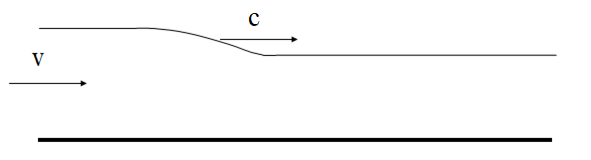
\includegraphics[scale=0.5]{./images/fr_waves_01.png}
	\caption{Wave in a channel showing velocities}
	\label{fig:fr01}
\end{figure}

The wave can be \textit{brought to rest} by subtracting the wave speed $-c$
	\begin{figure}[H]
	\centering
	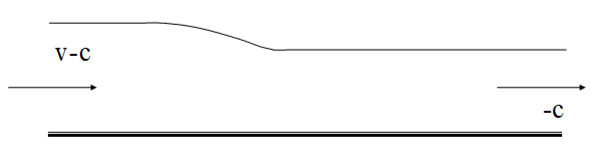
\includegraphics[scale=0.5]{./images/fr_waves_02.png}
	\caption{Wave in a channel \textit{brought to rest} }
	\label{fig:fr02}
\end{figure}
What is c, the speed of the wavefront?
Continuity:
\begin{equation*}
(v-c)(y+\delta y)=-cy
\end{equation*}
which gives
\begin{equation}
c\ \delta y = y v
\label{eq:cdy}
\end{equation}
Apply Newton’s Second Law:
\begin{align*}
\text{Total Force} &= \text{Pressure Force} \nonumber \\
\rho Q (V_2 - V_1) &= p_1 A_1 - p_2 A_2 \nonumber \\
\rho \left( (y_2\times 1 \times V_2) V_2 - (y_1 \times 1 \times V_1) V_1 \right) &= p_1 (y_1 \times 1) - p_2 (y_2 \times 1) \nonumber \\
\rho (y+\delta y)(c-v)^2 - \rho y c^2 &= \rho g \frac{y}{2}y -\rho g \frac{(y+\delta y)}{2}(y+\delta y) \nonumber \\ 
-gy\ \delta y &= c^2 \delta y - 2cvy \nonumber
\end{align*}
Using Eqn \ref{eq:cdy} gives
\begin{align}
-gy\ \delta y &= c^2 \delta y - 2c^2\ \delta y \nonumber \\
gy\ \delta y &= c^2\ \delta y \nonumber \\
c &= \sqrt{gy}
\end{align}
Hence Froude Number, 
\begin{equation}
Fr = \frac{v}{\sqrt{gy}} = \frac{v}{c} = \frac{\text{water speed}}{\text{wave speed}}
\end{equation}

If a pebble is dropped into a channel with flowing water, the pattern generated could be one of the following cases that represent the four types of flow.
	\begin{figure}[H]
	\centering
	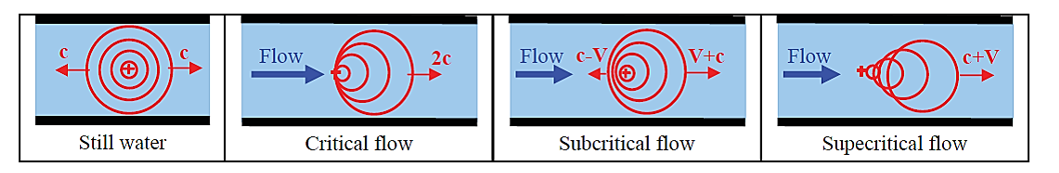
\includegraphics[scale=0.5]{./images/fr_pebble_waves.png}
	\caption{Wave patterns from a pebble thrown into water}
	\label{fig:fr03}
\end{figure}

Thus:

$Fr<1$ (slow flow)	wave speed $>$ water speed	a wave can travel upstream.

$Fr=1$(critical flow)	wave speed = water speed	a wave stays still in flow.

$Fr >1$ (fast flow)	wave speed $<$ water speed	a wave goes downstream only.

A reach of a channel which contains critical flow stops any disturbance in a downstream reach from travelling upstream to affect the reach upstream of the critical flow; essentially critical flow isolates effects parts of a channel from each other.

\newpage
\section{Uniform Flow in Open Channels}
\subsection{Uniform flow and the Development of Friction formulae}

When uniform flow occurs gravitational forces exactly balance the frictional resistance forces which apply as a shear force along the boundary (channel bed and walls).

\begin{figure}[H]
	\centering
	%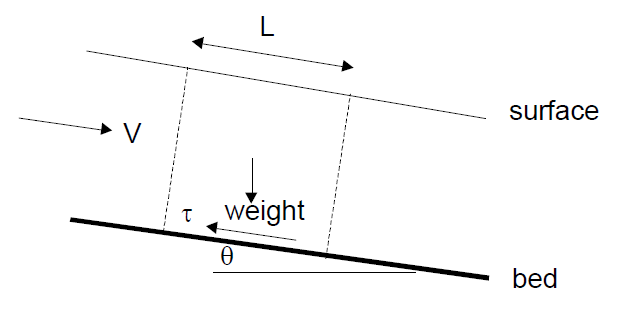
\includegraphics[scale=0.5]{./images/fig_171.png}
	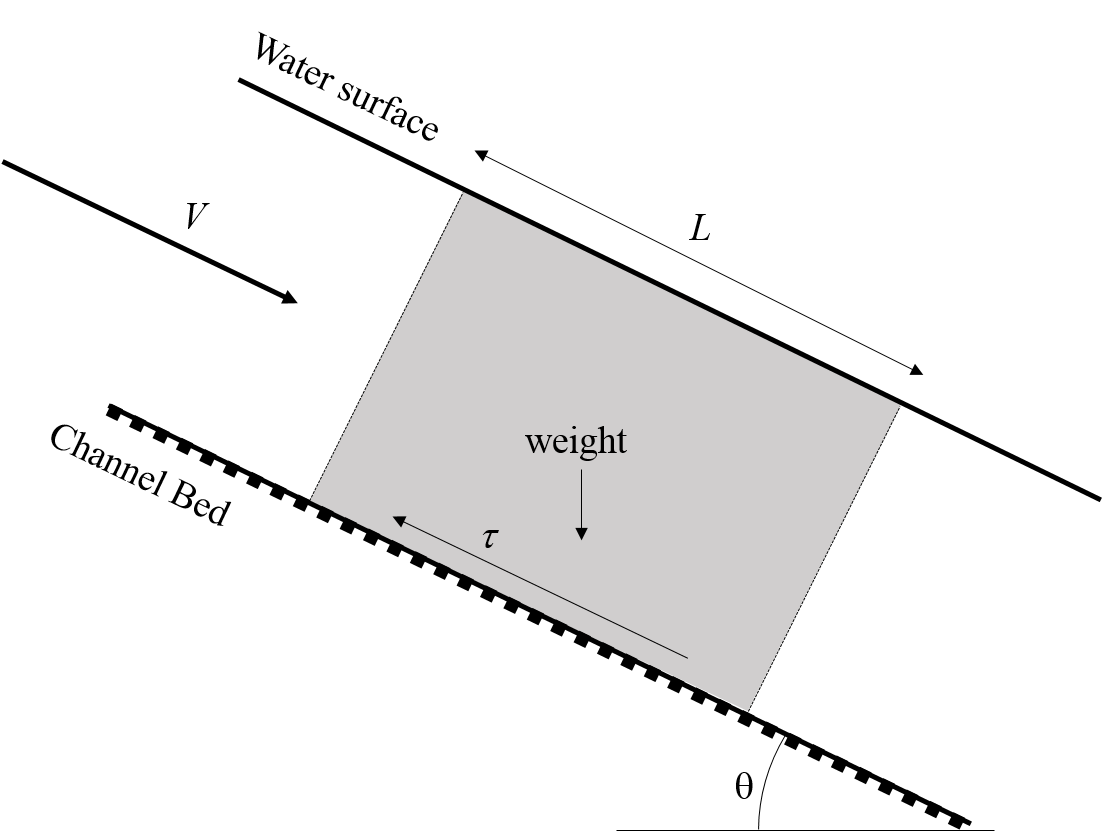
\includegraphics[scale=0.5]{./images/uniform_flow_section_2018.png}
	\caption{Forces on a channel length in uniform flow}
	\label{fig:171}
\end{figure} 
Considering figure \ref{fig:171}, the gravity force resolved in the direction of flow is

\begin{equation}
\text{gravity force} = \rho g A L \sin \theta
\end{equation}
 

and the boundary shear force resolved in the direction of flow is 

\begin{equation}
\text{shear force} = \tau_o P L
\end{equation}
 

In uniform flow these balance
 \begin{equation}
  \tau_o P L = \rho g A L \sin \theta
 \end{equation}
 


Considering a channel of small slope, then
 \begin{equation}
\sin \theta \approx \tan \theta = S_o
\end{equation}


So

 \begin{equation}
\tau_o = \frac{\rho g A S_o}{P} = \rho g R S_o
\label{eq:tau_o}
\end{equation}

\subsubsection{The Chezy equation}

If an estimate of $\tau_o$ can be made then we can make use of Equation \ref{eq:tau_o}.

If we assume the state of rough turbulent flow then we can also make the assumption the shear force is proportional to the flow velocity squared i.e.

 \begin{align*}
\tau_o &\propto V^2 \\
\tau_o &= K V^2
\end{align*}
 

Substituting this into equation \ref{eq:tau_o} gives


\begin{equation}
V = \sqrt{\frac{\rho g}{K}R S_o}
\end{equation} 

Or grouping the constants together as one equal to $C$
\begin{equation}
V = C\sqrt{R S_o}
\label{eq:chezy_v}
\end{equation} 

This is the Chezy equation and the $C$ the 'Chezy $C$'

In terms of $Q = (=AV)$ this is simply
\begin{equation}
Q = AC\sqrt{R S_o}
\label{eq:chezy_q}
\end{equation}

Because the $K$ is not constant the $C$ is not constant but depends on Reynolds number and boundary roughness (see discussion in previous section).

The relationship between $C$ and $\tau$ is easily seen be substituting equation \ref{eq:chezy_v} into the Darcy-Wiesbach equation written for open channels and is
\begin{equation}
C = \sqrt{\frac{2 g}{f}}
\end{equation} 
\subsection{The Manning equation}
A very many studies have been made of the evaluation of C for different natural and manmade channels. These have resulted in today most practising engineers use some form of this relationship to give $C$:

\begin{equation}
C = \frac{R^{1/6}}{n}
\label{eq:chezy_manning}
\end{equation}  

This is known as Manning's formula, and the $n$ as Manning's $n$.

Substituting equation \ref{eq:chezy_v} in to \ref{eq:chezy_manning} gives velocity of uniform flow:
\begin{equation}
V = \frac{R^{2/3}S_o^{1/2}}{n}
\label{eq:manning_v}
\end{equation} 
Or in terms of discharge
\begin{equation}
Q = \frac{1}{n}\frac{A^{5/3}}{P^{2/3}}S_o^{1/2}
\label{eq:manning_q} %eq 1.11
\end{equation} 


\textbf{Note:} \\
Several other names have been associated with the derivation of this formula - or ones similar and consequently in some countries the same equation is named after one of these people. Some of these names are; Strickler, Gauckler, Kutter, Gauguillet and Hagen.

The Manning's $n$ is also numerically identical to the Kutter $n$.

The Manning equation has the great benefits that it is simple, accurate and now due to it long extensive practical use, there exists a wealth of publicly available values of $n$ for a very wide range of channels.

Below is a table of a few typical values of Manning's $n$

\begin{table}[H]
	\centering
	\begin{tabular}{l|c|c}
		\hline
\textbf{Channel type}&\textbf{Surface material and form}&\textbf{Manning's $n$ range }\\
\hline
%\noalign{\vskip 2mm} 
River&earth, straight&0.02-0.025\\
&earth, meandering&0.03-0.05\\
&gravel (75-150mm), straight&0.03-0.04\\
&gravel (75-150mm), winding&0.04-0.08\\
\hline
unlined canal&earth, straight&0.018-0.025\\
&rock, straight&0.025-0.045\\
\hline
lined canal&concrete&0.012-0.017\\
\hline
lab. models&mortar&0.011-0.013\\
&Perspex& 0.009\\
\hline
\end{tabular}
\end{table}
	
\subsubsection{Conveyance}
Channel conveyance, K, is a measure of the carrying capacity of a channel. The $K$ is really an agglomeration of several terms in the Chezy or Manning's equation:
\begin{align}
Q &= AC\sqrt{R S_o} \nonumber \\
&= KS_o^{1/2}
\label{eq:manning_conveyance}
\end{align} 
 So
\begin{equation}
K = ACR^{1/2} = \frac{A^{5/3}}{n P^{2/3}}
\label{eq:conveyance}
\end{equation} 

Use of conveyance may be made when calculating discharge and stage in compound channels and also calculating the energy and momentum coefficients in this situation.

\subsection{\textit{Efficient} Uniform Flow Channels }

\textbf{What is the Best section?}

A channel can have many shapes and dimensions. However, certain types of channels are better at conveying flows than others.

Example: The following channels have the same amount of excavation (cross section area), as well as the same Manning’s n and bed slope. Which channel is the best hydraulically?

\begin{figure}[H]
	\centering
	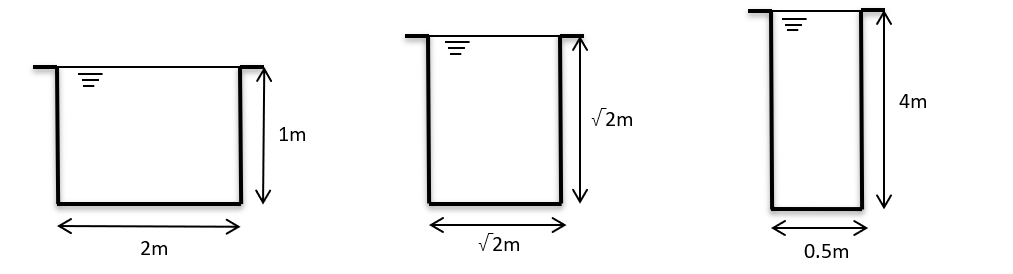
\includegraphics[scale=0.5]{./images/fig_best_sections.png}
	\caption{Channel Cross sections - which is the \textit{best}?}
	\label{fig:best_sections}
\end{figure}

Solution: 
Since

$P=b+2y$

$(a)=2+2 1=4m$

$(b)=2+2 2=4.24m$

$(c)=0.5+2 4=8.5m$
From
$Q=1/n A^(5/3)/P^(2/3) So=K/P^(2/3)$ (let $K=(A^(5/3)So)/n$)
Then
$Q_a=0.397K,Q_b=0.382K,Q_c=0.240K$
Hence a is the best and c is the worst.

A general pattern can be concluded from this example.

$Q=1/nA^(5/3)/P^(2/3) So$

The channel having the least wetted perimeter for a given area has the maximum conveyance; such a section is known as the best hydraulic section.

The derivation of the best hydraulic sections for some common shapes is illustrated here.


The design of a rigid (\emph{i.e.}, non-erodible) surface
open channel should be such that it is capable of carrying
maximum discharge with minimum excavation, construction, and
lining costs. This suggests that the designed
channel should have maximum hydraulic radius for a given
area or minimum perimeter for the given area since hydraulic
radius equals $A/P$. Therefore, a circular or semi-circular
section is the most efficient section. The adoption of
circular channel section is usually not feasible for sections larger than when a pipe could be used, due to the
difficulties of construction to achieves stable earth slopes
and other practical considerations. Hence, the designer has
to determine the most efficient section of a given shape. 
Considering a trapezoidal channel section, Fig. \ref{fig:section_trap_2018}, the
area of flow section $A$ and the wetted perimeter $P$ are given as
\begin{equation}
A = by + sy^2
\label{eq:1281}
\end{equation}
\begin{equation}
P = b +2y \sqrt{1 + s^2}
\label{eq:1282}
\end{equation}
Here,
\begin{equation*}
s = \cot \theta \qquad \qquad \text{or }  \qquad \qquad \frac{1}{s}= \tan\theta
\end{equation*}

\begin{figure}[H]
	\centering
	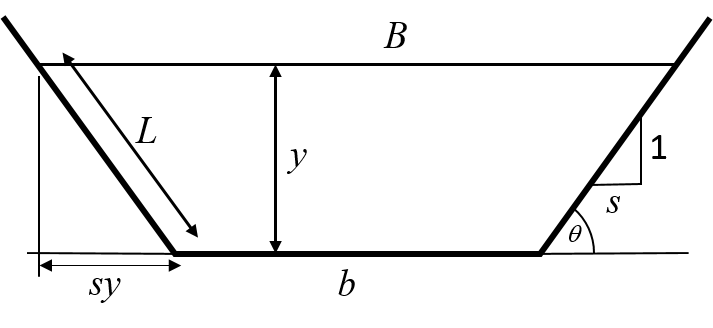
\includegraphics[width=8cm]{./images/section_trap_2018_a.png}
	\caption{A trapezoidal channel section}
	\label{fig:section_trap_2018}
\end{figure}
On substituting the value of $b$ obtained from Eq. \ref{eq:1281}
into Eq. \ref{eq:1282}, one gets
\begin{equation}
P = \frac{A}{y} - sy +2y \sqrt{1 + s^2}
\label{eq:1283}
\end{equation}	
To minimize $P$, evaluate $dP/dy$ with $A$ and $s$ constant
and set $dP/dy$ equal to zero. Therefore, 
\begin{equation*}
\frac{dP}{dy} = -\frac{A}{y^2} - z + 2 \sqrt{1 + s^2} = 0
\end{equation*}
or
\begin{equation}
A = y^2 \left [ 2 \sqrt{1 + s^2} - s \right ]
\label{eq:1284}
\end{equation}
Substituting the value of $A$ in Eq. \ref{eq:1284}, one gets 

\begin{equation*}
by + sy^2 = y^2 \left [ 2 \sqrt{1 + s^2} - s \right ]
\end{equation*}
$\therefore$
\begin{equation}
b = 2y  \left [ \sqrt{1 + s^2} - s \right ]
\label{eq:1285}
\end{equation}
Likewise, substituting the value of $A$ from Eq. \ref{eq:1284} in
Eq. \ref{eq:1283}, one gets

\begin{equation*}
P = y \left [ 2 \sqrt{1 + s^2} - s \right ] - sy + 2y \sqrt{1 + y^2}
\end{equation*}
or
\begin{equation}
P = 4y \sqrt{1 + s^2} - 2sy = 2y\left [ 2 \sqrt{1 + s^2} - s \right ]
\label{eq:1286}
\end{equation}
Thus,
\begin{equation}
R = \frac{A}{P} = \frac{y}{2}
\label{eq:1287}
\end{equation}
Equation  \ref{eq:1287} indicates that for any side slope $\theta$, 
the most efficient uniform flow channel of trapezoidal
shape would be the one for which hydraulic radius is
half the depth of flow. 

For a \textbf{rectangular} section, $\theta =$ 90 or $s=$ 0.
Therefore, the most efficient rectangular channel section
would be the one for which 
\begin{equation*}
A = 2y^2
\label{eq:1288}
\end{equation*}
\begin{equation}
P = 4y
\label{eq:1289}
\end{equation}
\begin{equation}
R = y/2
\label{eq:12810}
\end{equation}
and
\begin{equation}
B = 2y
\label{eq:12811a}
\end{equation}
To obtain the depth of flow for the most efficient section,
these equations must be solved in conjunction with
the Manning's equation.

Equations \ref{eq:1284}, \ref{eq:1287} are valid for any value of $s$.
The best value of $s$ for given $y$ and $A$ can be obtained
by setting $dP/ds$, evaluated from Eq. \ref{eq:1283}, equal to zero. 
\begin{equation*}
\frac{dP}{ds} = -y +2y\left [ \frac{1}{2} \frac{1}{\sqrt{1 + s^2}} \right ] 2s = 0
\end{equation*}
$\therefore$
\begin{equation*}
2s = \sqrt{1 + s^2}
\end{equation*}
$\therefore$
\begin{equation*}
s = \frac{1}{\sqrt{3}} = \cot \theta \qquad \qquad \text{or} \qquad\qquad \frac{1}{s} = \tan \theta = \sqrt{3}
\end{equation*}
$\therefore$
\begin{equation*}
\theta = 60^\circ
\end{equation*}
Thus, the maximum-flow trapezoidal section would be half of a hexagon.

Similarly, one can show that a circular channel section
running partially full would perform best when the depth of
flow is half the diameter. Geometric elements of the most
efficient channel sections of some selected shapes are given
in Table \ref{tab:1281}. Obviously, the semi-circular open channel
section is the best of all possible channel sections as it
gives minimum wetted perimeter for a given area of flow
section. However, the percentage increase in discharge for
semicircular section, compared to that in semi-hexagonal
section, is only small.

\begin{table}[H]
	\centering
	\begin{tabular}{ l llllll }
		\hline
		Cross-section & Normal & Area,  & Wetted  & Hydraulic  & Water surface  & Hydraulic \\
		& depth, $y_n$ & $A$ & perimeter, $P$ & radius, $R$ &  width, $B$ & depth, $D$\\
		\hline 
		Rectangular & $0.917 (Qn/\sqrt{S})^{3/8}$ & $2y^2$ & $4y$ & $0.500 y$ & $2y$ & $y$\\
		Triangle & $1.297 (Qn/\sqrt{S})^{3/8}$ & $y^2$ & $2.83 y$ & $0.354 y$ & $2y$ & $0.500y$\\
		(side slope 1:1) &  &  &  &  &   & \\
		Trapezoid  & $0.968 (Qn/\sqrt{S})^{3/8}$ & $1.73 y^2$ & $3.46 y$ & $0.500 y$ & $2.31 y$ & $0.750 y$\\
		(half of hexagon)  &  &  &  &  &   & \\
		Semicircle & $1.000 (Qn/\sqrt{S})^{3/8}$ &  $0.5\pi y^2$ & $\pi y$ & $0.500y$ & $2y$ & $0.250 \pi y$ \\
		Parabola  & $0.937 (Qn/\sqrt{S})^{3/8}$ & $1.89 y^2$ & $3.77 y$ & $0.500 y$ & $2.83 y$ & $0.667 y$\\
		$B  =  2\sqrt{2y}$ &  &  &  &  &  &   \\
		\hline
	\end{tabular}
	\caption{Geometric elements of the most efficient
		hydraulic sections \cite{french94}}
	\label{tab:1281}
\end{table}


\subsection{Computations in uniform flow}

We can use Manning's formula for discharge to calculate steady uniform flow. Two calculations are usually performed to solve uniform flow problems.
\begin{enumerate}
	\item Discharge from a given depth
	\item Depth for a given discharge
\end{enumerate}
In \underline{steady uniform flow the flow depth is know as normal depth}.

As we have already mentioned, and by definition, uniform flow can only occur in channels of constant cross-section (prismatic channels) so natural channel can be excluded. However we will need to use Manning's equation for gradually varied flow in natural channels - so application to natural/irregular channels will often be required.

\subsubsection{Uniform flow example 1 - Discharge from depth in a trapezoidal channel}

A concrete lined trapezoidal channel with uniform flow has a normal depth is 2m. 
The base width is $5m$ and the side slopes are equal at 1:2 (v:h, or $s=2$ in table \ref{tab:131})
Manning's $n$ can be taken as $0.015$, 
And the bed slope $S_o = 0.001$

What are:
\begin{enumerate}[label=\alph*]
	\item Discharge ($Q$)
	\item Mean velocity ($V$)
	\item Reynolds number ($R_e$)
\end{enumerate}
Calculate the section properties, using the appropriate geometrical formulae (e.g. table \ref{tab:131})

Area, $A =(b+sy)y$  
\begin{equation*}
A= (5 + 2y)y = 18m^2
\end{equation*}
Wetted perimeter, $P =b+2y\sqrt{1+s^2}$
\begin{equation*}
P= 5 + 2y\sqrt{1+2^2} = 13.94m
\end{equation*}
Use equation \ref{eq:manning_q} to get the discharge
\begin{align*}
Q &= \frac{1}{n}\frac{A^{5/3}}{P^{2/3}}S_o^{1/2} \\
&= \frac{1}{0.015}\frac{18^{5/3}}{13.94^{2/3}}0.001^{1/2}\\
& = 45 m^3/s
\end{align*}
Calculate the mean velocity using the continuity equation:
\begin{equation*}
V= \frac{Q}{A}=\frac{45}{18}=2.5 m/s
\end{equation*}
And the Reynolds, $R_e$, number (remember we use the hydraulic radius $R$  as the length scale), and so using $R=A/P$)
\begin{equation*}
R_e = \frac{\rho V R}{\mu} = \frac{\rho V}{\mu}\frac{A}{P} =\frac{1000 \times 2.5}{1.14\times 10^{-3} }\frac{18}{13.9} = 2.84 \times 10^6
\end{equation*}
This is very large - i.e. well into the turbulent zone - the application of the Manning's equation was therefore valid. 

What solution would we have obtained if we had used the Colebrook-White equation?

Probably very similar as we are well into the rough-turbulent zone where both equations are truly applicable.

To experiment an equivalent $k_s$ value can be calculated for the discharge calculated from $n = 0.015$  and $y = 2m$ [$k_s = 2.225mm$] (Use the Colebrook-White equation and the Darcy-Wiesbach equation of open channels - both given earlier). Then a range of depths can be chosen and the discharges calculated for these $n$ and $k_s$ values. Comparing these discharge calculations will give some idea of the relative differences - they will be very similar.


\subsubsection{Uniform flow example 2 - Depth from Discharge in a trapezoidal channel}

Using the same channel as above, if the discharge is know to be $30m^3/s$ in uniform flow, what is the normal depth?

Again use equation \ref{eq:manning_q} 

Area, $A =(b+sy)y$  \\
Wetted perimeter, $P =b+2y\sqrt{1+s^2}$
\begin{align*}
Q &= \frac{1}{0.015}\frac{((5+2y)y)^{5/3}}{\left(2+2y\sqrt{1+2^2}\right)^{2/3}}0.001^{1/2}\\
30 &= 2.108\frac{((5+2y)y)^{5/3}}{\left(2+2y\sqrt{1+2^2}\right)^{2/3}}
\end{align*}
We need to calculate $y$ from this equation (and remember that this is \textbf{normal depth} so $y = y_n$. 

Even for this quite simple geometry the equation we need to solve for normal depth is complex. 

One simple strategy to solve this is to try some trial values of $y$ and calculate the right hand side of this equation and compare it to $Q (=30)$ on the left. When it equals $Q$ we have the correct $y$. Even though there will be several solutions to this equation, this strategy generally works because we have a good idea of what the depth should be (e.g. it will always be positive and often in the range of $0.5 \text{ to } 10 m$). 

In this case from the previous example we know that at $Q = 45 m^3/s$, $y = 2m$. So at $Q = 30 m^3/s3 then 3y < 2.0m$.

\begin{table}[H]
	\centering
	\begin{tabular}{cc}
		\hline
		Trials of $y$ ($m$) &Discharge $Q$ ($m^3/s$) \\
		\hline
		1.7	&32.7\\
		1.6	&29.1\\
		1.63&	30.1\\
		\hline
	\end{tabular}
	\caption{Trials of $y$}
	\label{tab:ex21}
\end{table}

\subsubsection{Uniform flow example 3 -Calculation of niform Flow and Froude Number}
Find the discharge in a channel that is flowing with uniform flow of depth 3m, as shown below, and has a bed slope S0=  1 in 1000 and a Chezy C of 45 m1/2/s. Is this flow sub or supercritical?

Uniform flow and friction specified by the Chezy friction factor, so use the Chezy Equation

	\begin{figure}[H]
	\centering
	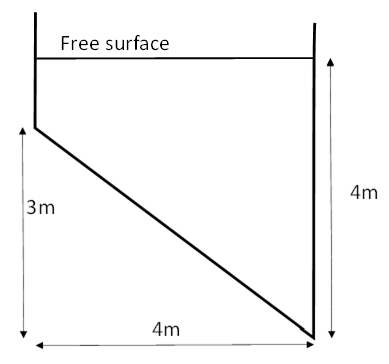
\includegraphics[scale=0.5]{./images/fr_eg_01.png}
	\caption{Channel Cross section}
	\label{fig:fr_eg_01}
\end{figure}
$Q=AV=AC(RS_o )$

Slope: $S_o=1/1000=0.001v$

Flow area: $A=((3 4))/2+1 4=10 m^2$

Wetted perimeter: $P=1+(3^2+4^2 )+4=10m$

Hydraulic radius: $R=A/P=1m$

Hydraulic mean depth: $D_m=A/B=10/4=2.5m$

$Q=10 45(1 0.001)=14.23 m^3/s$ this is the discharge in the channel

$V=Q/A=14.23/10=1.423m/s$ this is the velocity of flow

$Fr=V/ (gD_m )=1.423/(9.8 2.5)=0.287$ this is $< 1$, so it is sub critical flow.

\subsubsection{Uniform flow example 4 - A compound channel}

If the channel in the above example were to be designed for flooding it may have a section like this:

\begin{figure}[H]
	\centering
	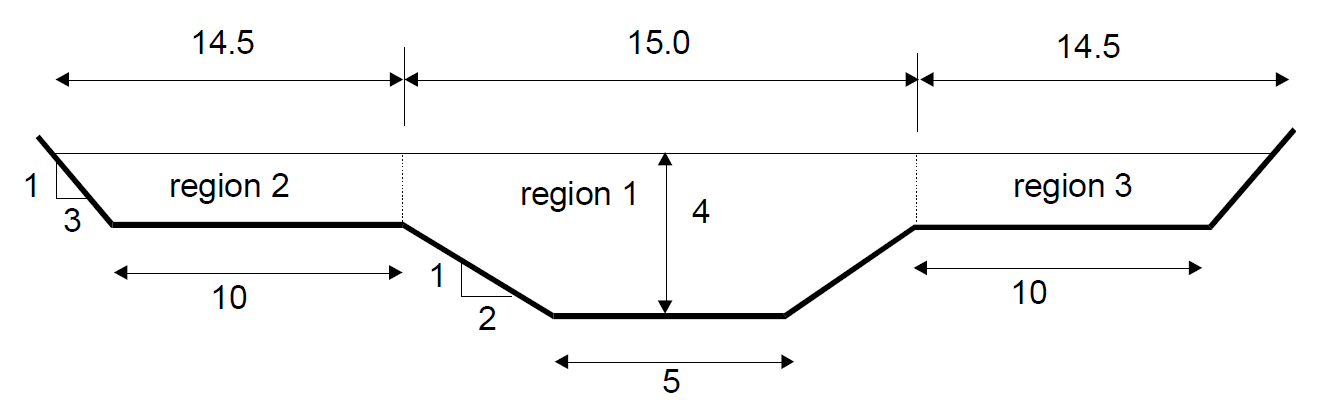
\includegraphics[scale=0.5]{./images/fig_eg41.png}
	\caption{A Compound section}
	\label{fig:eg41}
\end{figure}
When the flow goes over the top of the trapezoidal channel it moves to the "flood plains" so the section allows for a lot more discharge to be carried.

If the flood channels are 10m wide and have side slopes of $1:3$, and the Manning $n$ on these banks is $0.035$, what are
\begin{enumerate}[label=\alph*,noitemsep]
	\item the discharge for a flood level of $4m$?
	\item the energy coefficient ?
\end{enumerate}
First split the section as shown in to three regions (this is arbitrary - left to the engineers judgement). 
Then apply Manning's formula for each section to give three discharge value and the total discharge will be $Q = Q_1 + Q_2 + Q_3$.

Calculate the properties of each region:
\begin{equation*}
A_1 = \left( \frac{5+15}{2}\right)2.5+(15 \times 1.5) = 47.5m^2
\end{equation*}
\begin{equation*}
A_2 = A_3 = \left( \frac{10+14.5}{2}\right)1.5 = 18.38m^2
\end{equation*}
\begin{equation*}
P_1 = 5 + \left(2 \sqrt{5}\times 2.5\right) = 16.18m
\end{equation*}
\begin{equation*}
P_2 = P_3=10 + \left(1.5 \sqrt{10}\times \right) = 14.75m
\end{equation*}
The conveyance for each region may be calculated from equation \ref{eq:conveyance}
\begin{equation*}
K_1 =\frac{47.5^{5/3}}{0.015 \times 16.18^{2/3}} = 6492.5
\end{equation*}
\begin{equation*}
K_2 = K_3 =\frac{18.38^{5/3}}{0.035 \times 14.74^{2/3}} = 608.4
\end{equation*}


And from Equation \ref{eq:manning_q} or Equation \ref{eq:manning_conveyance}
the discharges
\begin{equation*}
Q_1 = \frac{1}{0.015}\frac{47.5^{5/3}}{16.18^{2/3}}0.001^{1/2}
\end{equation*}
or
\begin{equation*}
Q_1 = K_1 0.001^{1/2}= 205.3 m^3/s
\end{equation*}
And
\begin{equation*}
Q_2 = Q_3 = \frac{1}{0.035}\frac{18.38^{5/3}}{14.74^{2/3}}0.001^{1/2}
\end{equation*}
or
\begin{equation*}
Q_2=Q_3 = K_2 0.001^{1/2}= 19.2 m^3/s
\end{equation*}
So
\begin{equation*}
Q = Q_1 + Q_2 + Q_3 = 243.7 m^3/s
\end{equation*}
The velocities can be obtained from the continuity equation:
\begin{equation*}
V_1 = \frac{Q_1}{A_1} = 4.32 m/s
\end{equation*}
\begin{equation*}
V_2 = V_3 = \frac{Q_2}{A_2} = 1.04 m/s
\end{equation*}
And the energy coefficient may be obtained from Equation \ref{eq:alpha}
\begin{equation*}
\alpha = \frac{\int u^3 \; dA}{\overline{V}^3 \; A} = \frac{V_1^3 A_1+ V_2^3 A_2+V_3^3 A_3}{\overline{V}^3(A_1+A_2+A_3)} 
\end{equation*}
where
\begin{equation*}
\overline{V} = \frac{Q}{A} = \frac{V_1 A_1+ V_2 A_2+V_3 A_3}{A_1+A_2+A_3} 
\end{equation*} 
Giving 
\begin{equation*}
\alpha = 1.9
\end{equation*}


This is a \textbf{very high} value of $\alpha$ and a clear case of where a velocity coefficient should be used.

Note that this method does not give completely accurate relationship between stage and discharge because some of the assumption are not accurate. E.g. the arbitrarily splitting in to regions of fixed Manning $n$ is probably not what is occurring in the actual channel. However it will give a good estimate as long as care is taken in choosing these regions.

\section{Examples: Uniform Flow in Open Channels}
\textbf{Solutions can be found on Minerva}

\begin{enumerate}
	\item	A concrete, trapezoidal channel has a bottom slope of So = 0.0009 and a Manning roughness factor of n = 0.013. The bottom width of the channel is b = 2.5m, and the side slopes are 1 in 2. Determine the velocity and discharge when the flow is normal at a depth of 1.8m. 
	
	\item	A trapezoidal channel has a bottom slope of slope of So = 1 in 40 and a Manning roughness factor of n = 0.016. The bottom width of the channel is b = 6.0m, and the side slopes are 1 in 3. Determine the normal depth in this channel for Q = 42.3m3/s.  
	
	\item	A trapezoidal channel has side slopes of 1:3/4 and the slope of the bed is 1 in 2000. Determine the optimum dimensions of the channel if it is to carry water at 0.5m3/s. Use the Chezy formula, assuming that C = 80m1/2/s.
	
	\item \label{eg:04}	The cross section of a stream can be approximated by the compound channel shown in the figure below. The bottom slope is So = 0.0009. The Manning roughness factor n = 0.025 for the main channel and n = 0.035 for the overbank areas. Determine the normal depth for a discharge of 197m3/s. 
		\begin{figure}[H]
		\centering
		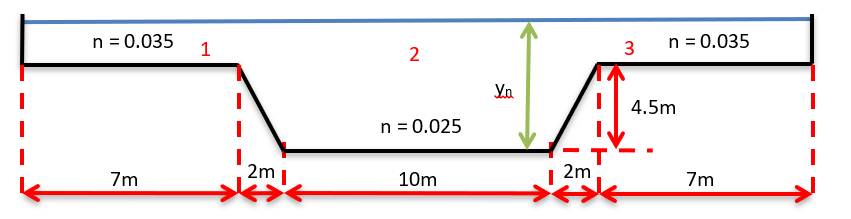
\includegraphics[scale=0.5]{./images/fig_eg4.png}
		\caption{A Compound section}
		\label{fig:eg4}
	\end{figure}
	\item	The width of the channel considered in Question \ref{eg:04} will be reduced; however, this reduction must not cause an increase of more than 0.15m in the flow depth for the discharge of 197m3/s. The encroachment will be over a long distance, and we can assume that normal flow will occur throughout the encroachment portion of the channel. Determine the minimum allowable channel width, b. 
	
	\item	The flow discharge through a rectangular channel 4.6m wide is 11.3m3/s when the slope is 1:100. Is the flow subcritical or supercritical? The Manning roughness coefficient is n = 0.012.
	
	\item	An open channel with n = 0.011 is to be designed to carry 1.0m3/s of water at a slope of 0.0065. Find the most efficient cross section for a rectangular section. 
	
\end{enumerate}

\begin{thebibliography}{99}
\bibitem{chow59} Chow, VT, \emph{Open-Channel Hydraulics,} McGraw-Hill Book Co., 1959.
\bibitem{chadwick} Chadwick, A, and Morfett, J, \emph{Hydraulics in Civil and Environmental Engineering}, 2nd Ed, E \& FN Spon, 1993.
\bibitem{french94}	French, RH: Open-Channel Hydraulics, McGraw-Hill Book Co., 1994.
\end{thebibliography}
\end{document}